% This is lnbip.tex the demonstration file of the LaTeX macro package for
% Lecture Notes in Business Information Processing from Springer-Verlag.
% It serves as a template for authors as well.
% version 1.0 for LaTeX2e
%
\documentclass[lnbip]{svmultln}
%
\usepackage{makeidx}  % allows for indexgeneration
\makeindex          % be prepared for an author index
%

\usepackage{color}
\usepackage{amsmath}
\usepackage{amsfonts}
\usepackage{amssymb}
\usepackage{graphicx}
%\usepackage{amsthm}
\usepackage{epsfig} 
\usepackage{lipsum}
\usepackage{float}
\usepackage{pdfpages}
\usepackage{wrapfig}
\usepackage{graphicx} 
\usepackage{subfig}  


\usepackage{natbib}
\bibliographystyle{abbrvnat}
%\setcitestyle{authoryear,open={((},close={))}} 



\newcommand{\myfloatalign}{\centering}

\newcommand{\ie}{i.\,e. }
\newcommand{\Ie}{I.\,e. }
\newcommand{\eg}{e.\,g. }
\newcommand{\Eg}{E.\,g. } 

\setlength{\textheight}{22 cm}
\setlength{\textwidth}{14 cm}



\begin{document}
%
\mainmatter              % start of the contribution
%
\title{Study of the best stochastic gradient descent optimizers for automatic license plate recognition}

%\title{Minimization of learning errors for automatic license plate recognition}
%
\titlerunning{Stochastic gradient for alpr}  % abbreviated title (for running head)
%                                     also used for the TOC unless
%                                     \toctitle is used
%
\author{Hassan T. Kajila\inst{1} \and Jordan Masakuna\inst{5}  \and Geysla Memita\inst{2} \and Godwill Ilunga\inst{3} \and August Muhau\inst{4}}
%
\authorrunning{Hassan Kajila et al.}   % abbreviated author list (for running head)
%
%%%% list of authors for the TOC (use if author list has to be modified)
\tocauthor{Hassan Kajila, Jordan Masakuna, Geysla Memita, Godwill Ilunga, August Muhau}
%
\institute{Université Nouveaux Horizons, Faculté des Sciences Informatiques, Lubumbashi, DR of Congo
	\\ email: \texttt{contact@hassankajila.com}
	\and
	Université Nouveaux Horizons, Faculté des Sciences Informatiques, Lubumbashi, DR of Congo
	\\ email: \texttt{geysla.memita@unhorizons.org}
	\and
	Université Nouveaux Horizons, Faculté des Sciences Informatiques, Lubumbashi, DR of Congo
	\\ email: \texttt{godwill.ilunga@unhorizons.org}
	\and
	Université Nouveaux Horizons, Département des Sciences de base, Lubumbashi, DR of Congo
	\\ email: \texttt{august.muhau@unhorizons.org}
	\and
	Université de Kinshasa, Département des Sciences Informatiques, Kinshasa, DR of Congo
	\\ email: \texttt{jordan.masakuna@unikin.ac.cd}
}
	
\maketitle              % typeset the title of the contribution
 \index{Kajila, Hassan} % entries for the author index
 \index{Sungu, Pascal}  % of the whole volume
 \index{Ilunga, Godwill}
 \index{Muhau, August}
 \index{Masakuna, Jordan}
 \index{Memita, Geysla}
 
 %\vspace{0.3cm}
\begin{abstract}        % give a summary of your paper
	%Nowadays, a huge number of cameras are deployed exclusively for surveillance. The contents of images and videos are often interpreted by human operators. 
	Nowadays, a lot of cameras are deployed exclusively for surveillance.
	This makes content tracking and analysis so expensive, not to mention the mistakes that human fatigue and carelessness can introduce.
	In this work we propose a method, based on artificial intelligence, which allows computer systems to derive meaningful information from digital images. As part of this work, the aim is to perform automatic license plate recognition using optimizers based on the \emph{stochastic gradient descent}.
	Therefore, the main objective of this present study is to examine the different optimizers and determine the best able to recognize license plates, in spite of possible geometric transformations, in order to reduce the constraints in the detection of license plates as to the position of the camera. 
	%Experiments on several license plates that undergo a slight geometric transformation, in image, made it possible to validate the performance obtained with this approach.
	Experiments on several license plates made it possible to validate the performance obtained with this approach.
%                         please supply keywords within your abstract
\keywords{Supervised learning, Stochastic optimization methods, Stochastic gradient descent, Visual Geometry Group (VGG), Automatic License Plate Recognition, Geometric transformations.}
\end{abstract}

%\vspace{0.2cm}

%
\section{Introduction}
%
	%In this paper, it is a question of approaching the use of the algorithms of numerical optimization, precisely of minimization of the errors. 
	
	% Learning Error
	
	The first untrained model built in supervised learning to perform a certain task usually does not yield an accurate result compared to the output or task it was supposed to do \cite[]{goodfellow2016deep, geron2017hands}.
	The loss function (also called cost function) is a way to measure whether the model better schematizes the system it's supposed to describe. This is necessary to determine the deviation, or learning error, %error rate,
	between the current output of model and its expected output \cite[]{antoine2018apprentissage}. 
	%
	For example for classification tasks, a learning error %error rate 
	for a binary SVM (Support Vector Machine) classifier might be reported, although the loss function used to train the SVM only very loosely models the number of errors on the training set, and similarly neural net training uses convex costs, such as mean square error or cross-entropy \cite[]{burges2006learning}.  
	%
	Thus often in machine learning tasks, there are actually two cost functions: the desired cost, and the one used in the optimization process. \\
	
	% Minimisation
	Minimizing errors or optimizing weight parameters for a neural network is an important task in the learning process. The training dataset for object detection problems are typically very large and the capabilities of machine learning methods are limited by computation time rather than sample size. % \cite{bottou2010large}.
	%new
	For deep convolutional networks trained in a supervised setting, the training objective is typically the minimization of learning error (\eg classification error see \cite[chap. 3]{ml2008python}) at the top network layer. \\Many neural network training algorithms explicitly minimize a loss function. For instance, the back-propagation technique uses the gradient descent algorithm to minimize the mean squared error (MSE see \cite[]{bosman2020visualising}) loss function. 
	%new
	Deep convolutional neural networks trained using back-propagation are thus achieving record performance in a variety of large-scale computer vision tasks \cite[]{krizhevsky2012imagenet, simonyan2014very, huang2017densely}.\\
	
	% Objectif
	This paper deals with the use of numerical optimization algorithms, precisely the minimization of errors. They will be applied to machine learning that will enable computer systems to automatically recognize vehicle license plates. This work will be done using optimizers focused on stochastic gradient descent to optimize the parameters of the convolutional neural network (CNN).
	Therefore for each algorithm or optimizer, their efficiency will be examined and compared with each other, and classified according to the score (accuracy, loss) obtained.\\
	
	% Division
	We discuss the stochastic gradient descent (SGD) method in section 2. We describe the proposed CNN dataset and model built with the VGG architecture in section 3 and quantitatively evaluate the performance of different SGD-based optimizers. And also we present the results of the application in automatic license plate recognition in section 4. We present our findings and an in-depth discussion on the performance of the best optimizers in section 5.
	

\section{Minimization by the stochastic descent gradient}
	%Preliminary
	The loss function, as mentioned in the introduction, is a way to measure whether the algorithm has done a good job.  
	Let the following e.g (from \cite[]{bottou1991stochastic}), Consider a function, $J(z,w)$, that measures the cost incurred by a system defined by some parameter $w$ processing an observation $z$. In the case of connectionist learning, this function is equal to $(y-f(x,w))^2$ (with $f(x,w) = w^Tx$) and measures how well the output $y$ for pattern $x$ is approached. Learning consists of finding the parameter $w*$ that minimizes the following cost:
	
	\begin{equation}
		Q(w) = \ell(J(z,w)) = \int J(z,w)dP(z)
	\end{equation}
	%The brackets denote the average value, over all possible examples, of the squared difference
	%between the output and the actual class.
	
	$dP$ is an unknown probability distribution which characterizes the problem to learn, and $J$, the loss function, describes the learning system itself.\\
	
	%Many connectionist learning algorithms consists of minimizing a cost of the form
	%Gradient descent
	Gradient descent refers to a first-order iterative optimization algorithm for finding a local minimum of a differentiable function. It performs a minimization optimization by following the negative of the downward gradient of the loss function to locate the minimum thereof. This algorithm requires a starting point in the problem, such as a randomly selected point in the input space \cite[]{bottou2012stochastic}.
	The gradient descent will find the minimum of the loss function $\ell \in \mathbb{R}$ starting from the random parameters $w_i$a which will be the initial coordinates.
	
	The optimizers based on gradient stochastic are more used in neural network weights optimization \cite[]{ruder2016overview}.
	Gradient descent takes the loss function $\ell = Q(w)$ parameterized by the parameters of the model $w \in \mathbb{R}^d$ and minimizes it by updating the parameters in the opposite direction to the gradient of the loss function. It's a way to convert add $\nabla_w Q(w)$ to the parameters. The learning rate $\eta$ determines the step size required to reach the local minimum. In other words, it follows the direction of the slope of the surface produced by the downward loss function until it reaches a minimum \cite[]{bottou1991stochastic, ruder2016overview}. Minimizing the cost, see equation \ref{eq:cost}, apparently is not a difficult problem. If the training set is finite, the distribution $dP(z)$ is discrete, and we can explicitly apply the gradient descent algorithm. Each iteration involves a sum over the N examples $z_i$. Let the following equation:
	\begin{equation}
	w_{t+1}   = w_t - \eta_t {\nabla_w Q(w_t)} 
	 = w_t - \eta_t \int \nabla_w J(z,w_t) dP(z) 
	 = w_t - \eta_t \frac{1}{N} \sum_{i=1}^{N}  \nabla_w J(z_i,w_t)	
	\label{eq:descent_gradient}
	\end{equation}
	A stochastic process ${w_t; t=1,...N}$ depends on the randomly selected sample at each iteration.
	The stochastic gradient descent directly optimizes the expected risk, since the examples are randomly drawn from the ground truth distribution \cite[]{bottou2010large}.
	However, stochastic gradient descent algorithm have proven to be faster, more reliable, and less likely to hit bad local minima than standard gradient descent methods \cite[]{wijnhoven2010fast}. The algorithm updates the weights according to the gradient of the loss function after each example is presented \cite[]{bottou1991stochastic}.\\
	
	SGD has difficulty navigating through cost function valleys, i.e. areas where the surface curves much more steeply in one dimension than another, which are common around local optima \cite[]{antoine2018apprentissage}. In these scenarios, SGD oscillates on the slopes of the valley while making only a hesitant progression along the bottom towards the local optimum \cite[]{ruder2016overview,bottou1991stochastic}.
	It's about to solve this problem of oscillation that we resort to the various optimizers, always focused on the SGD, which proposes an improvement of the traditional SGD by playing the various parameters and hyperparameters of this one \cite[]{lin2019nesterov,ruder2016overview}.
	
	%In the following, for the comparative study, we will select the faster SGD optimizers according to \cite[]{geron2017hands, bottou2012stochastic}, and that are widely used in Deep Learning to deal with the aforementioned challenges
	
	In the following, for the comparative study, we will select the fastest SGD optimizers variants which are widely used in Deep Learning, according to \cite[]{geron2017hands, bottou2012stochastic}, to deal with the above-mentioned challenges \cite[]{ruder2016overview}. 
	optimizer: Adaptive Gradient or AdaGrad \cite[]{lydia2019adagrad}, Root Mean Squared Propagation or RMSprop \cite[]{geron2017hands}, Adaptive Moment Estimation or Adam \cite[]{kingma2014adam} and Nesterov-accelerated Adaptive Moment Estimation or Nadam \cite[]{lin2019nesterov,dozat2016incorporating}.


\section{Dataset \& Training Model }
\subsection{Data Preprocessing}
	%The Training dataset was build with a dataset of 450 license plate images and xml annotations file. Labeling is done with the LabelImg tool, which is a graphical image annotation tool. The dataset 	is divided into three subsets proportionally: 70\% for training, 10\% for validation, 20\% for testing.
	
	%The training dataset was built with a dataset of 450 images of license plates and xml annotation files. The work is done with LabelImg, a graphical image annotation tool. The dataset is divided into three subsets proportionally: 70\% for training, 10\% for validation, 20\% for testing.
	
	The training set was built with a dataset of 450 license plate images and an xml annotation file. Image labeling is done with LabelImg, which is a graphical image annotation tool. The dataset is divided into three subsets: 70\% for training, 10\% for validation, and 20\% for testing.
	


\subsection{Build the CNN model with VGGNet architecture}

	%\begin{wrapfigure}{r}{0.5\textwidth}
	%	\myfloatalign{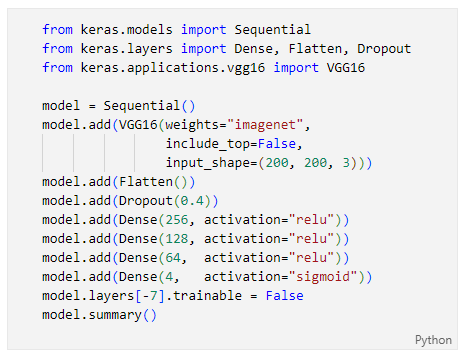
\includegraphics[width=\linewidth]{images/cnn_model}}
	%	\caption[]{}\label{fig:relu}
	%\end{wrapfigure}
	
	VGG stand for Visual Geometry Group \cite[][chap. 10]{antoine2018apprentissage}, it is a standard deep Convolutional Neural Network architecture with multiple layers. VGG competed in ILSVRC 2014, got good classification rate. Today VGGNet is a family of deep neural networks (from A to E). The VGG is the basis of revolutionary object recognition models \cite[]{tammina2019transfer}.  
	
 	First a \textbf{"Sequential"} model is created in which we add \textbf{VGG-16} (\ie with 16 layers, see \cite[]{antoine2018apprentissage, geron2017hands}) as the first layer. The VGG-16 will take as input arrays of size $(200 \times 200 \times 3)$ which correspond to the reduced size of the images of the dataset (reduced in the preprocessing stage).
 	The VGG-16 output is flattened with the \textbf{Flatten} layer. Finally, 4 layers \textbf{Dense}, are added later, and will act as completely connected layers with as output an array of size $(4 \times 1)$ which corresponds to the 4 points which will allow the model to draw the rectangle that will frame the license plate in the image.
 	
	\begin{table}[H]
		\centering
		\begin{tabular}{lll}
			\hline
			{\texttt{Layer (type)}} & 
			{\texttt{Output Shape}} & 
			{\texttt{Param \#}} \\
			\hline
			\hline
			%& & \\
			\texttt{vgg16 (Functional) } &  \texttt{(None, 6, 6, 512) } & \texttt{14714688} \\
			
			\texttt{flatten (Flatten)}  & \texttt{(None, 18432)} & \texttt{0} \\ 
			
			\texttt{dropout (Dropout)} & \texttt{(None, 18432)} & \texttt{0} \\ 
			
			\texttt{dense (Dense)} & \texttt{(None, 256)} & \texttt{4718848 }\\
			
			\texttt{dense\_1 (Dense)} & \texttt{(None, 128)} & \texttt{32896} \\
			
			\texttt{dense\_2 (Dense)} & \texttt{(None, 64)} & \texttt{8256} \\ 
			
			\texttt{dense\_3 (Dense)} & \texttt{(None, 4)} & \texttt{260}  \\
			\hline
			\hline
			\multicolumn{3}{l}{
				\begin{tabular}{l}
					\texttt{Total params: 19,474,948} \\
					\texttt {Trainable params: 4,760,260} \\
					\texttt {Non-trainable params: 14,714,688} \\
				\end{tabular}
			}\\
			\hline
			
		\end{tabular}
		\caption[]{The information the convolutional neural network builds with VGG-16.}
		\label{tab:vgg-16}
	\end{table}
	In this section, we will first explore and evaluate an architecture of convolutional neural networks, the Visual Geometry Group. The developed model, VGG-16, contains \texttt{19,474,948} parameters (fewer parameters compared to VGG-19) and about \texttt{4.7} million parameters are exploitable (optimizable).
	

	%\subsection{Training} % talk about : Trainable params: 4,760,260
	

	


%
\section{Result \& discussion}
%	
	%The are made using python tensorflow according to \cite{geron2017hands} for ???
	\subsection{Optimizer evaluation}
	\subsubsection*{\qquad \textbullet \ \textbf{SGD}}:
	The SGD minimizes the model parameter with a score of 67.5\% accuracy and about 1\% error. And on the validation data, the accuracy is 72.7\% and an error of 1.2\%. The test result reveals an error of 0.73\% and an accuracy of 79.3\%. 

	
	\begin{table}[H]
		\centering
		\begin{tabular}{l|l|l}
			\hline
			\textbf{Training} & \textbf{Validation} & \textbf{Test} \\
			%& & \\
			\hline
			
			\texttt{loss: 0.0105} & \texttt{loss: 0.0120} & \texttt{loss: 0.00732} \\
			\texttt{accuracy: 0.6755} & \texttt{accuracy: 0.7273} & \texttt{accuracy: 0.7931} \\
			
			\hline
			
		\end{tabular}
	\end{table}
	
	\begin{figure}[H]
		\myfloatalign
		\subfloat[SGD loss]
		{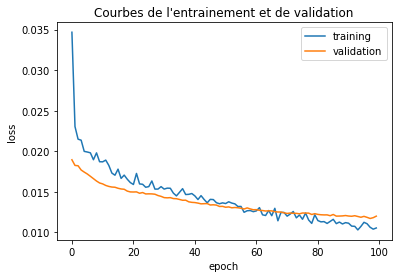
\includegraphics[width=.40\linewidth]{images/sgd_loss_curve}} \quad
		\subfloat[SGD accuracy]
		{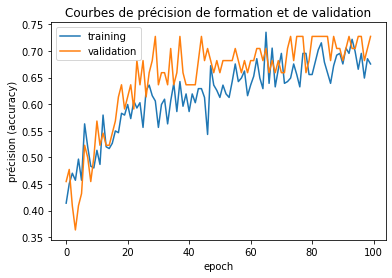
\includegraphics[width=.40\linewidth]{images/sgd_accuracy_curve}} 
		
		\caption{Accuracy and loss graph for SGD.}
	\end{figure}

	
	\subsubsection*{\qquad \textbullet \ \textbf{RMSprop}}:
	The model minimized with the RMSprop gives a score of 95.7\% accuracy, displays a deviation of about 28.2\% compared to the SGD, and 0.044\%. The error and accuracy rate of RMSpro in validation is 1\% and 77.2\% respectively. The RMSprop optimizer also shows a lower error percentage than the SGD.\\
	The convergence of RMSprop is rather accentuated because the minimization stabilizes after 80 steps and reaches the minimum value at the 110th step.
	\begin{table}[H]
		\centering
		\begin{tabular}{l|l|l}
			\hline
			\textbf{Training} & \textbf{Validation} & \textbf{Test} \\
			%& & \\
			\hline
			
			\texttt{loss: 4.4475e-04} & \texttt{loss: 0.0109} & \texttt{loss : 0.005589} \\
			\texttt{accuracy: 0.9570} & \texttt{accuracy: 0.7727} & \texttt{accuracy : 0.8505} \\
			
			\hline
			
		\end{tabular}
	\end{table}
	\begin{figure}[H]
		
		\subfloat[RMSprop loss]
		{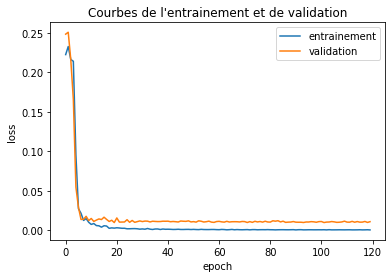
\includegraphics[width=.4\linewidth]{images/rmsprop_loss_curve}} \quad
		\subfloat[RMSprop accuracy]
		{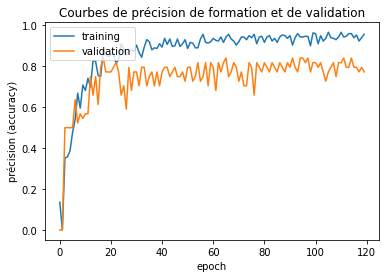
\includegraphics[width=.4\linewidth]{images/rmsprop_accuracy_curve}} 
		
		\caption{Accuracy and loss graph for RMSprop.}
		\label{fig:1}
	\end{figure}
	
	
	\subsubsection*{\qquad \textbullet \ \textbf{AdaGrad}}:
	AdaGrad scored poorly compared to the previous optimizer, RMSprop. An error rate of 1.2\% and accuracy of 62.9\% is the score of the AdaGrad optimizer. After $120$ steps, which is the maximum step set for the tests, the minimization still does not stabilize. The minimum values are reached at the level of the $80th$ step.
	\begin{table}[H]
		\centering
		\begin{tabular}{l|l|l}
			\hline
			{\textbf{Training}} & {\textbf{Validation}} & {\textbf{Test}} \\
			\hline
			\texttt{loss: 0.0124} & \texttt{loss: 0.0156} & \texttt{loss: 0.0094} \\
			\texttt{accuracy: 0.6291} & \texttt{accuracy: 0.6591} & \texttt{accuracy: 0.5747} \\
			\hline
		\end{tabular}
	\end{table}
	\begin{figure}[H]
		\myfloatalign
		\subfloat[AdaGrad loss]
		{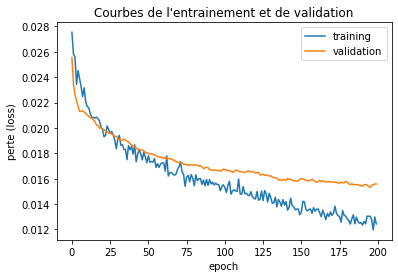
\includegraphics[width=.4\linewidth]{images/adagrad_loss_curve}} \quad
		\subfloat[AdaGrad accuracy]
		{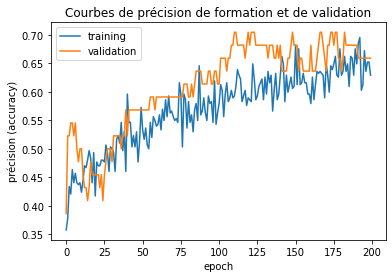
\includegraphics[width=.4\linewidth]{images/adagrad_accuracy_curve.png}} 

		\caption[]{Accuracy and loss graph for Adagrad.}
	\end{figure}
	
	
	\subsubsection*{\qquad \textbullet \ \textbf{Adam}}:
	The Adam forms a model with 92.3\% accuracy and an error of 0.086\%, a bit higher compared to RMSprop. The validation score is 81.8\% accuracy and 1.1\% error. After the tests, 83.9\% accuracy and 0.05\% error is the observed score. RMSprop minimizes the cost better and shows a nice score compared to Adam.
	\begin{table}[H]
		\centering
		\begin{tabular}{l|l|l}
			\hline
			\textbf{Training} & \textbf{Validation} & \textbf{Test} \\
			\hline
			\texttt{loss: 8.6163e-04} & \texttt{loss: 0.0110} & \texttt{loss : 0.00526} \\
			\texttt{accuracy: 0.9238} & \texttt{accuracy: 0.8182} & \texttt{accuracy : 0.8390} \\
			\hline
		\end{tabular}
	\end{table}
	\begin{figure}[H]
		\myfloatalign
		\subfloat[Adam loss]
		{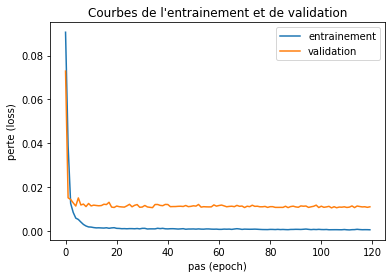
\includegraphics[width=.4\linewidth]{images/adam_loss_curve_3}} \quad
		\subfloat[Adam accuracy]
		{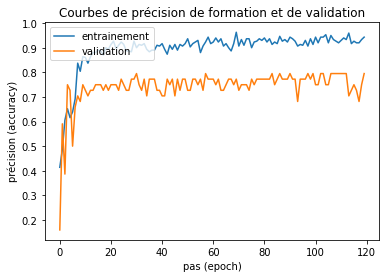
\includegraphics[width=.4\linewidth]{images/adam_accuracy_curve_3}} 
		
		\caption[]{Accuracy and loss graph for Adam.}
	\end{figure}

	
	
	\subsubsection*{\qquad \textbullet \ \textbf{Nadam}}:
	Nadam, (Nesterov-accelerated Adaptive Moment Estimation), 
	is an extension of the Adam optimizer to which we add the Nesterov Accelerated Gradient (NAG) \cite[]{ruder2016overview}.
	Nadam shows an attractive performance (from training, validation and testing point of view) compared to other optimizers studied in this work. It gives, as result, an accuracy of 95.3\%  and an error of 0.04\%. Nadam accelerates the speed of convergence in a drastic way, it stabilizes at 30 steps and reaches the minimum value in only 40 steps.
	
	\begin{table}[H]
		\centering
		\begin{tabular}{l|l|l}
			\hline
			\textbf{Training} & \textbf{Validation} & \textbf{Test} \\
			%& & \\
			\hline
			\texttt{loss: 4.6549e-04} & \texttt{loss: 0.0109} & \texttt{loss : 0.00479} \\
			\texttt{accuracy: 0.9536} & \texttt{accuracy: 0.7955 }& \texttt{accuracy : 0.9080}\\
			
			\hline 
			
		\end{tabular}
	\end{table}
	
	\begin{figure}[H]
		\myfloatalign
		\subfloat[Nadam loss]
		{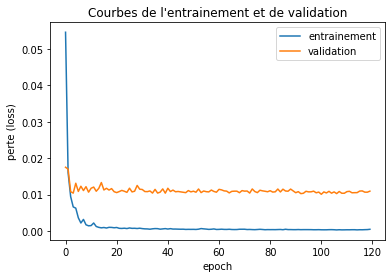
\includegraphics[width=.4\linewidth]{images/nadam_loss_curve}} \quad
		\subfloat[Nadam accuracy]
		{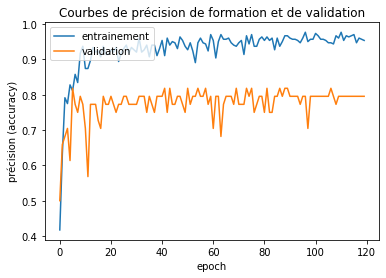
\includegraphics[width=.4\linewidth]{images/nadam_accuracy_curve}} 
		
		\caption[]{Accuracy and loss graph for Nadam}
	\end{figure}
	RMSprop gives very low error in training compared to other optimizers, in testing phase Adam reveals lower error than RMSprop. The optimizer which has a good average, in the 3 phase, is Nadam with very good precision.
	
	
	\subsection{Optimizer classify  according to ALPR} %optimizer classify according to alpr
	
	This work admits the Nadam optimizer as an algorithm that best minimizes errors and obtains a good score, in the context of ALPR, compared to the other optimizers studied. Below is a list of the best minimizing optimizers (table \ref{tab:error_rank}), ranked in descending order, for the case of the automatic license plate recognition problem.
		\begin{table}[H]
			\centering
			\begin{tabular}{|l|l|l|l|}
				\hline
				\textbf{N\textdegree} & \textbf{Training} & \textbf{Validation} & \textbf{Test} \\
				\hline
				
				\textbf{1. RMSprop} &
				\texttt{0.0004447} &
				\texttt{0.0109} &
				\texttt{0.005597} \\
				\hline
				
				\textbf{2. Nadam} &
				\texttt{0.00046549} &
				\texttt{0.0109} &
				\texttt{0.00479} \\
				\hline
				
				\textbf{3. Adam} &
				\texttt{0.00086163} &
				\texttt{0.0110} &
				\texttt{0.00526} \\
				\hline
				
				\textbf{4. Adagrad} &
				\texttt{0.0124} &
				\texttt{0.0156} &
				\texttt{0.0094} \\
				\hline
				
				\textbf{5. SGD} &
				\texttt{0.0105} &
				\texttt{0.0120} &
				\texttt{0.00732} \\
				\hline
			\end{tabular} 
		\caption{Table showing error rate per optimizer, listed in descending order. }
		\label{tab:error_rank}
		\end{table}	
		The top 3 optimizers (from table \ref{tab:accuracy_rank}) served as tests in license plate detection despite the geometric transformation, i.e. the 3 models that had a good training, validation and test score.
		\begin{table}[H]
			\centering
			\begin{tabular}{|l|r|r|r|}
				\hline
				& \textbf{Training} & \textbf{Validation} & \textbf{Test} \\
				
				\hline
				\textbf{Nadam} &
				\texttt{95.36\%} &
				\texttt{79.55\%} &
				\texttt{90.80\%} \\
				\hline
				\textbf{Adam} &
				\texttt{92.58\%} &
				\texttt{81.82\%} &
				\texttt{83.90\%} \\
				\hline
				\textbf{RMSprop} &
				\texttt{95.70\%} &
				\texttt{77.27\%} &
				\texttt{85.05\%} \\
				\hline
				%& & & \\
				%\hline
				%& & & \\
				%\hline
				
			\end{tabular}
		\caption{Table illustrating the resulting accuracy by the 3 best optimizer.} 
		\label{tab:accuracy_rank}
		\end{table}
	
	
	
	%\begin{figure}[H]%bth
	%	\centering
	%	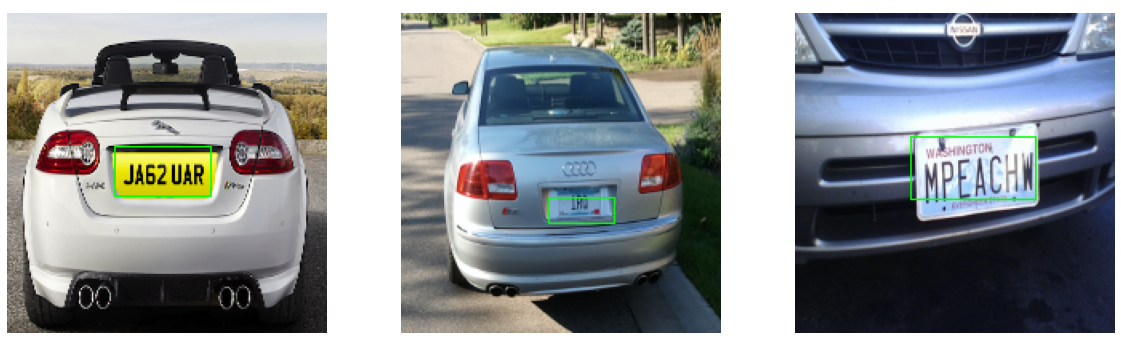
\includegraphics[width=\textwidth]{images/predicted_trans_image_2}
	%	%\caption{}
	%	\caption{The plates are recognized.}
	%	\label{fig:predicted_trans_image_2}
	%\end{figure}

	\begin{figure}[H]%bth
		\centering
		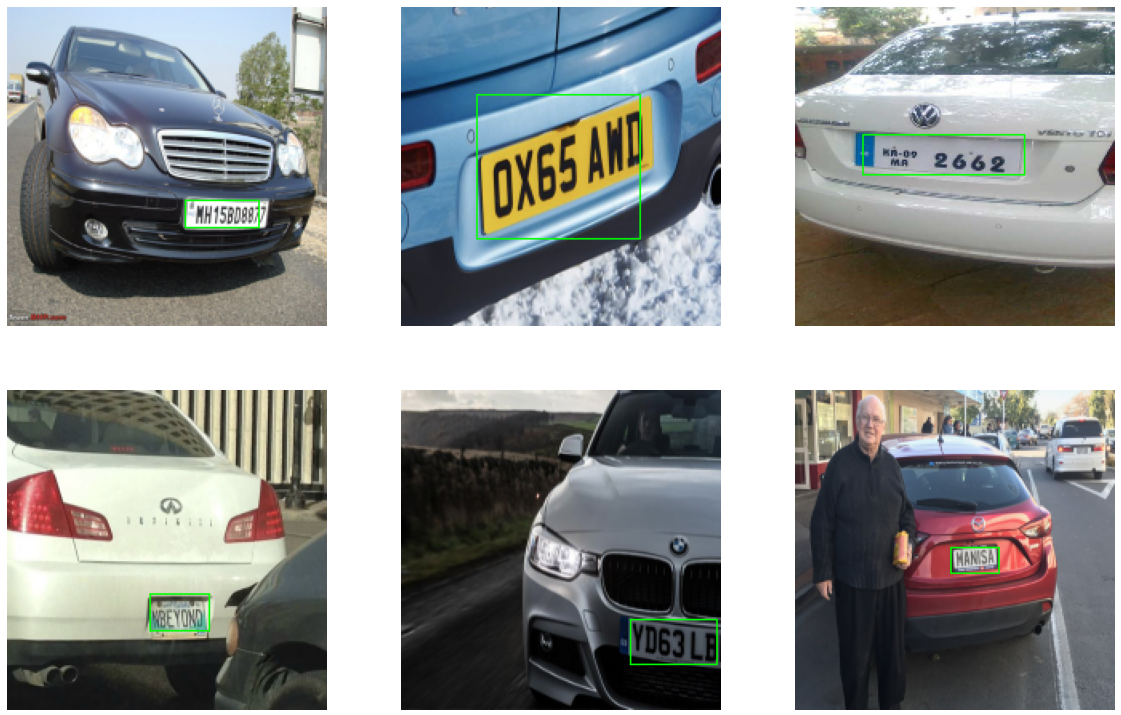
\includegraphics[width=0.75\textwidth]{images/predicted_trans_image_1}
		\caption{The plates recognized despite the slight geometric transformation.}
		\label{fig:predicted_trans_image_1}
	\end{figure}

	\subsection{Optical Character Recognition}
	
	After recognizing the license plate,
	with the OpenCV Python library properties, it will be easy to extract the region of interest on the image which is the detected plate in the green rectangle. OCR processing is performed on the area, as shown in figure \ref{fig:ocr_result}.
	
	The result returned by EasyOCR Reader is an array containing a tuple of size 3, and the value we are interested in is at position 2 which corresponds to index 1 (\texttt{result[0][1]}).
	
	\noindent\texttt{result = [([[0, 0], [70, 0], [70, 17], [0, 17]], 'Wor 5i6k', 0.49005824012267324)]}
	
	\noindent The result in the \texttt{[Wor 5i6k]} terminal corresponds to the registered license plate number.

	\begin{figure}[H]%bth
		\centering
		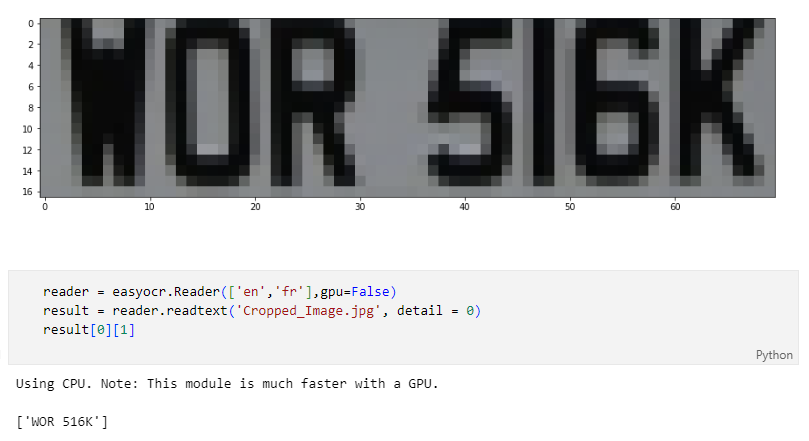
\includegraphics[width=\textwidth]{images/ocr_result}
		%\caption{}
		\caption{The result of character recognition.}
		\label{fig:ocr_result}
	\end{figure}
	
	
	\section{Conclusion}
	
	This paper provides an answer to our problem. It was a question of explaining when the minimization of errors in learning occurs. In order to justify the comparative study made, which made it possible to determine which optimizer is suitable for the problem of license plate detection in an image.
	
	The conclusive results of the experiment, presented in section 4, show the performance of different optimizers treated in this work. The 3 best optimizers identified were used in license plate recognition. The RMSprop optimizer showed its feat in minimizing the cost function well compared to Nadam or Adam but from the precision point of view the Nadam optimizer came out first for this problem of the APLR.
	
	



%



%
% ---- Bibliography ----
%
%\bibliographystyle{plain}
%\nocite{*}
\bibliography{myref}
%
\end{document}
